% !TeX program = tectonic
% ---------------------------------------------------------------------------
% Laya Football Evaluation — protocol preprint (registered report, stage 1)
% Compile:  cd paper && tectonic main.tex
% Author:   [AUTHOR NAME] — placeholders to be replaced before submission.
% ---------------------------------------------------------------------------
\documentclass[11pt]{article}

\usepackage[margin=1in]{geometry}
\usepackage{amsmath,amssymb}
\usepackage{newtxtext,newtxmath}
\usepackage{booktabs}
\usepackage{array}
\usepackage{xcolor}
\usepackage{graphicx}
\usepackage{caption}
\usepackage{tikz}
\usetikzlibrary{arrows.meta,positioning}
\usepackage{enumitem}
\usepackage{microtype}
\usepackage[numbers,sort&compress]{natbib}
\usepackage[colorlinks=true,allcolors=blue!45!black]{hyperref}
\usepackage{fancyhdr}

% ---- Visible placeholders (replace before submission) ----------------------
\newcommand{\AuthorName}{[AUTHOR NAME]}
\newcommand{\Affil}{[AFFILIATION]}
\newcommand{\GitHubURL}{[GITHUB URL]}
\newcommand{\OsfDOI}{[OSF DOI]}
\newcommand{\ArxivID}{[ARXIV ID]}

% ---- Header / footer -------------------------------------------------------
\pagestyle{fancy}
\fancyhf{}
\fancyhead[L]{\small Laya Football Evaluation --- Preregistered Protocol}
\fancyhead[R]{\small\thepage}
\renewcommand{\headrulewidth}{0.4pt}

\captionsetup{font=small,labelfont=bf}

\newcommand{\eps}{\varepsilon}

\title{\textbf{Laya as a Real-Time Probabilistic Decision Engine for Football:\\
A Preregistered Multi-Agent Evaluation Protocol}}

\author{\AuthorName\thanks{Corresponding author: \AuthorName, \Affil.
Text licensed CC-BY 4.0; code licensed MIT.}\\[2pt]
{\small \Affil}}

\date{September 26, 2026}

\begin{document}

\maketitle
\thispagestyle{fancy}

\begin{center}
\small\itshape
Study protocol v2.0.0 --- Registered-report stage 1 (design paper; no results).
\\
Preregistration: \OsfDOI{} \quad$\cdot$\quad Code: \GitHubURL{} \quad$\cdot$\quad Preprint: \ArxivID{}
\end{center}
\vspace{2pt}

\begin{abstract}
\noindent
AI agents built on large language models are increasingly deployed as decision
engines that return full probability distributions on demand, yet their quality
as \emph{live} probabilistic forecasters is rarely measured with the rigor
applied to statistical models. We present a preregistered evaluation protocol
(v2.0.0) for Laya, a typed, multilingual AI decision engine, as a real-time
probabilistic forecaster of football match outcomes. At every snapshot---taken
at seven fixed cutoffs (pre-match and minutes 15, 30, 45, 60, 75, 85) and
immediately after salient events (goals, red cards, penalties,
substitutions)---Laya emits distributions over the final 1X2 result, 17 score
buckets, total corners (0--20, 21+), and total yellow cards (0--12, 13+). The
protocol enforces point-in-time integrity: automated leakage tests on 100\,\% of
snapshots, forbidden-field and provenance checks, and three information tiers
(A: pre-match; B: minimal live; C: full live). Laya is compared with baselines
receiving \emph{identical} information---uniform, historical frequency, Poisson,
Dixon--Coles, multinomial logistic regression, and bookmaker odds---under a
strict temporal split, with a stratified bootstrap clustered by match (at least
2{,}000 replicates) and Holm--Bonferroni correction, against five preregistered
hypotheses (H1--H5). This article reports the protocol only; data collection,
execution, and results follow in stage~2. The reference implementation is open
source (MIT); the text is CC-BY 4.0.
\end{abstract}

\vspace{4pt}
\noindent\textbf{Keywords:} probabilistic forecasting; calibration; large
language models; sports analytics; preregistration; evaluation protocol;
multi-agent systems.

\section{Introduction}
\label{sec:intro}

Good decisions in dynamic environments require continuously updated
\emph{distributions}, not one-off point estimates. A decision-maker monitoring
a live process needs $P(\text{outcome} \mid \text{information available now})$,
refreshed every time new information arrives, and needs to know whether those
probabilities can be trusted---that is, whether they are calibrated, sharp, and
reactive to events. The statistical literature provides mature tools for
judging such forecasts: proper scoring rules \citep{brier1950,gneiting2007},
calibration--sharpness diagnostics \citep{gneiting2007b,murphy1973}, and
clustered inference for dependent observations \citep{cameron2015}.

A new class of systems now claims a place in this pipeline: AI decision engines
built on large language models (LLMs) that return structured probability
distributions over typed outcome spaces, on demand and in natural language.
Their measured quality as \emph{repeated, in-play probability assessors} is,
however, largely unknown. Existing LLM evaluations emphasize accuracy on
static question sets \citep{hendrycks2021} or one-shot forecasting tournaments
\citep{halawi2024,schoenegger2024}; they rarely enforce that the model sees
only information that was available at prediction time, rarely sample the same
process at many instants, and rarely compare against statistical baselines
receiving exactly the same information. Live football forecasting is an
unforgiving testbed for exactly these properties: targets are objectively
defined, information arrives as a dense event stream, and the risk of post-hoc
contamination---through data sources that silently encode final results---is
pervasive.

This paper presents the design of a study that addresses this gap. We evaluate
\emph{Laya}, a typed, multilingual AI decision engine exposed through a
software development kit (SDK), as a real-time probabilistic forecaster of
football match outcomes: the final 1X2 result, the final score grouped into 17
buckets, total corners, and total yellow cards. The evaluation is
\emph{multi-instant}: each match is sampled at fixed cutoffs (pre-match, 15,
30, 45, 60, 75, 85 minutes) and immediately after salient events (goals, red
cards, penalties, substitutions). It is \emph{leakage-audited}: point-in-time
integrity is enforced by construction and verified by automated tests executed
on 100\,\% of snapshots. It is \emph{fair}: every baseline receives the same
information tier as Laya at the same cutoff. And it is
\emph{preregistered}: hypotheses, metrics, baselines, and blocking thresholds
were frozen in this protocol before any test-set analysis, following
open-science practice \citep{nosek2018,osc2015}.

Our contributions are:
\begin{enumerate}[leftmargin=1.6em,itemsep=1pt]
  \item a preregistered, fully reproducible evaluation protocol (v2.0.0) for an
        AI decision engine as a \emph{multi-instant} probabilistic forecaster,
        with typed tasks, information tiers, and leakage tests on every
        snapshot;
  \item an audit-first data architecture: immutable raw artifacts, deterministic
        SHA-256 identifiers, versioned state snapshots, and error-coded
        validity handling;
  \item a nine-agent reference implementation whose agents communicate
        exclusively through hashed, versioned artifacts, enabling idempotent
        re-execution and third-party audit;
  \item an open-source release (MIT code, CC-BY 4.0 text) that generalizes to
        other typed decision engines and other dynamic domains.
\end{enumerate}

This document is the design paper (registered-report stage 1). It deliberately
reports no empirical results; all results will be reported in stage~2 exactly
as specified here, and analyses not specified here will be labeled exploratory.

\section{Related Work}
\label{sec:related}

\paragraph{Statistical models of football outcomes.}
The reference models for association-football scores are decades old and
remain strong. \citet{maher1982} introduced independent Poisson models for
home and away goals; \citet{dixon1997} corrected the low-score dependence and
introduced time-decayed maximum-likelihood estimation; \citet{karlis2003}
developed bivariate Poisson models for sports data; \citet{rue2000} framed
league prediction in a Bayesian dynamic model. For \emph{in-play} forecasting,
\citet{dixon1998} modeled the arrival of goals as a birth process with
score-dependent intensities---an explicit model of how a distribution should
evolve as the match unfolds, which is precisely the behavior we probe with
event-driven snapshots. Corners and cards are less studied but are count
variables for which Poisson and negative-binomial machinery applies directly.

\paragraph{Evaluating probabilistic forecasts.}
Brier's 1950 score \citep{brier1950} and its decomposition
\citep{murphy1973} inaugurated distributional verification; the unified
treatment of proper scoring rules by \citet{gneiting2007} and the
calibration--sharpness principle of \citet{gneiting2007b} define modern
practice. For the ordered three-class 1X2 outcome, the ranked probability score
is the natural strictly proper choice \citep{gneiting2007}. Calibration of
predicted probabilities is usually summarized by the expected calibration
error (ECE), whose binning choices are known to matter
\citep{naeini2015,guo2017}. For count targets, \citet{czado2009} introduced the
randomized probability integral transform (PIT) to correct the discreteness of
PIT histograms, and discrete CRPS and log-score implementations are available
in standard software \citep{jordan2019}. Bookmaker odds are strong,
hard-to-beat benchmarks when converted to implied probabilities with a
margin-removal method fixed in advance \citep{spann2009}. Because snapshots of
the same match share one realized outcome, our uncertainty quantification
clusters at the match level, using bootstrap resampling of clusters
\citep{efron1979,cameron2015}.

\paragraph{LLMs as probability assessors.}
Large-scale benchmarks measure the accuracy of LLM answers
\citep{hendrycks2021} but not the calibration of the full distributions they
can be asked to output. A growing literature elicits verbalized or numerical
confidence \citep{lin2022,xiong2024} and reports promising aggregate accuracy
in forecasting tournaments \citep{halawi2024,schoenegger2024}. What is missing
is an evaluation of an LLM-based \emph{engine}, queried repeatedly during a
live process, under strict point-in-time information control, against matched
statistical baselines, and with preregistered hypotheses. Our protocol imports
the evaluation standards of the forecasting literature---proper scores,
randomized PIT, coverage, clustered inference, and multiplicity control---into
that setting.

\paragraph{Open science and preregistration.}
Large-scale replication failures \citep{osc2015} motivated preregistration and
registered reports as a governance mechanism for confirmatory research
\citep{nosek2018}. We adopt the same discipline for an AI evaluation:
hypotheses H1--H5, primary metrics, baseline definitions, split design, and
blocking thresholds are frozen before the test set is inspected; this paper is
the stage-1 (design) document of that registered report.

\section{The Laya System Under Test}
\label{sec:laya}

Laya\footnote{Laya is a third-party AI decision engine; it is evaluated as-is
and is not modified by this study.} is a typed decision engine exposed through
an SDK and a router that returns \emph{structured probability distributions},
not free-form text. Two task types cover our targets: \texttt{choice}, which
returns a categorical distribution over a versioned list of criteria, and
\texttt{score}, which returns a distribution over an ordered support that may
include a tail category (e.g., ``21+''). The multilingual variant is used;
canonical questions are written in English, and their exact wording, order,
and category names are versioned---any change creates a new task version.

Three properties govern how the system enters the evaluation.

\paragraph{(i) Version pinning.}
Before any data collection, the following are recorded and frozen in the
experiment manifest: exact package name and installed version, checkpoint hash
or identifier, the engine variant used (the base or the multilingual one), maximum
context length, Python version and dependency lockfile, router configuration,
inference parameters (including any seed and batch settings), run identifier,
and execution date. Architectural characteristics announced in vendor
documentation are \emph{not} treated as experimental facts until verified in
the installed environment. The pinned version is used for all confirmatory
analyses.

\paragraph{(ii) Contract validation before scale-up.}
A smoke test precedes collection and verifies: the real import name; the
actual signature of the prediction entry point; the types accepted by the
\texttt{questions} argument; the output format; the behavior on an invalid
question; the reproducibility of two identical requests; and the conservation
of probabilities and output keys. A deterministic repetition audit is then run
on a stratified sample of at least 10\,\% of snapshots with $k=5$ identical
requests: if outputs are identical, a single query suffices in production; if
they differ, either $k=5$ is used for all snapshots of the main protocol, or a
frozen aggregation rule is adopted \emph{before} the test set---individual
outputs are always retained. Inter-call variance, decision-flip frequency,
and log-loss variation are reported.

\paragraph{(iii) Typed outputs and secondary confidence.}
Every response is stored raw (with hash) before parsing. Parsing succeeds only
if the payload is valid JSON, contains exactly the documented keys, has finite
probabilities in $[0,1]$ summing to one within $10^{-6}$, and has no missing
or duplicate category; the expected value must be coherent with the declared
tail convention. A failed validation is recorded with an error code and never
silently repaired or renormalized. The \emph{confidence} value optionally
returned by Laya is a secondary output: it is stored and analyzed separately
(calibration of confidence against the correctness of the most probable
decision, and its relation to log loss), but it never substitutes for a
probability in any metric. High confidence is not evidence of accuracy.

\section{Evaluation Protocol}
\label{sec:protocol}

\subsection{Research questions and preregistered hypotheses}
\label{sec:hyp}

The primary question is: \emph{at a cutoff $t$, given only information
available at $t$, does Laya produce predictive distributions that are better
calibrated and/or more discriminative than the predefined baselines} for the
final 1X2 result, the grouped final score, total corners, and total yellow
cards? Secondary questions address improvement with match progression,
reaction to salient events, stability under paraphrase and reordering, the
information level required for a given quality, error concentration across
matches and strata, and calibration-versus-discrimination trade-offs.

Five hypotheses are preregistered and must appear in the experiment manifest
before the final test set is evaluated (Table~\ref{tab:hyp}). Any hypothesis
not preregistered is exploratory and will be presented as such.

\begin{table}[t]
\centering
\small
\begin{tabular}{@{}p{0.9cm}p{2.6cm}p{11.2cm}@{}}
\toprule
\textbf{ID} & \textbf{Theme} & \textbf{Statement} \\
\midrule
H1 & Temporal progression & The 1X2 log loss decreases as the cutoff moves from
pre-match to 85 minutes. \\
H2 & Calibration & Laya's calibration (ECE and log loss) is better than that
of the historical-frequency baseline at identical information. \\
H3 & Event reaction & After a goal, the probability of the corresponding
winner increases on average, all else equal. \\
H4 & Robustness & Semantically equivalent paraphrases do not strongly modify
the predictive distribution. \\
H5 & Counts & For corners and cards, Laya is compared separately against (a) a
historical-mean baseline and (b) an adapted count model. \\
\bottomrule
\end{tabular}
\caption{Preregistered confirmatory hypotheses (H1--H5).}
\label{tab:hyp}
\end{table}

\subsection{Data scope, sources, and conventions}
\label{sec:data}

The scope is five competitions---Premier League, La Liga, Serie A, Bundesliga,
Ligue 1---over three complete seasons defined explicitly in
\texttt{experiment\_manifest.json}, with a power-oriented target of
approximately 1{,}000 included matches. This figure is a power objective, not a
quota: matches of insufficient quality are excluded, and the final counts of
included, excluded, and missing matches are reported per competition and
season.

One primary source is chosen before collection (candidates include
StatsBomb, API-Football, FBref, or another documented source, subject to
license verification); a secondary source verifies results and events but never
silently completes the primary one. Every source record stores the provider,
endpoint or file, source identifier, retrieval date, HTTP status or error
code, SHA-256 hash of the raw content, and known license restrictions.

\emph{Inclusion} requires: an officially finished match; no extra time; the
final score present; events and statistics sufficient for the targets;
timestamps precise enough for the cutoffs; and uniquely resolved home/away
identities. \emph{Exclusion with logging} applies to: stopped, postponed,
replayed, or abandoned matches; extra time or shootouts; inconsistencies
between final score and events; missing targets; impossible timestamps;
unresolved duplicates; and post-match-only aggregates used where a live
snapshot would be required. Excluded matches are never replaced after
consulting results.

Counting conventions follow the protocol: goals---including penalties and own
goals---count for the benefiting team in the official 90-minute-plus-stoppage
score; shootout goals are not match goals; corners are counted per team and
aggregated; yellow cards attributed to players on the pitch count toward the
target, while cards shown to coaches, staff, substitutes, and the bench are
excluded; a second yellow to the same player counts as such only where the
source reliably supports it (with a preregistered sensitivity analysis);
duplicate events are deduplicated on a documented key, never by untraceable
manual deletion.

\subsection{Targets and typed tasks}
\label{sec:targets}

Table~\ref{tab:targets} summarizes the four primary tasks. The 1X2
distribution is derived from the joint score distribution,
\begin{equation}
P(1)=\sum_{h>a}P(h,a),\qquad
P(X)=\sum_{h=a}P(h,a),\qquad
P(2)=\sum_{h<a}P(h,a),
\end{equation}
using the 90-minute-plus-stoppage score without extra time or shootouts. The
grouped-score task uses 17 ordered buckets: the 16 exact scores with both
components in $\{0,1,2,3\}$ and an \texttt{other} bucket collecting any score
with a component above 3. Because of the \texttt{other} class, this task is
never described as an exact-score distribution. For higher resolution on
goals, two separate marginal tasks (home goals and away goals, each 0--7 plus
8+) are added; these marginals are never recombined into a joint distribution
without an explicitly validated method.

\begin{table}[t]
\centering
\small
\begin{tabular}{@{}llll@{}}
\toprule
\textbf{Task} & \textbf{Type} & \textbf{Support} & \textbf{Tail} \\
\midrule
1X2 final result      & derived from score & home / draw / away & --- \\
Grouped final score   & \texttt{choice}   & 16 exact scores $+$ \texttt{other} (17) & \texttt{other} \\
Total corners         & \texttt{score}    & $0,\dots,20$ & $21+$ \\
Total yellow cards    & \texttt{score}    & $0,\dots,12$ & $13+$ \\
\bottomrule
\end{tabular}
\caption{Primary prediction targets. Question wording, criteria lists, and
their order are versioned; any modification creates a new task version.}
\label{tab:targets}
\end{table}

Corners use levels $0$--$20$ plus a $21+$ tail; yellow cards use $0$--$12$ plus
$13+$. If the SDK cannot express an ordered tail class, the preregistered
fallback is a censored target $\min(\text{total},20)$ (respectively
$\min(\text{total},12)$), and expected values are then reported as censored
expectations, never presented as uncensored. Tail thresholds may be raised
\emph{before} the experiment if descriptive analysis shows excessive tail
mass; they may never be chosen after comparing results.

\subsection{Snapshot plan and information tiers}
\label{sec:snapshots}

Two families of snapshots sample each match. \emph{Fixed} snapshots are taken
at pre-match and at minutes 15, 30, 45, 60, 75, and 85
(\texttt{cutoffs\_seconds} $=[0,900,1800,2700,3600,4500,5100]$), created only
if the match is still in progress at the corresponding instant; the 45-minute
snapshot represents the state at the end of the first period before interval
events, unless a documented decision states otherwise.
\emph{Event-driven} snapshots are created immediately after every goal, red
card, penalty (awarded or taken), and substitution; event type, timestamp,
and identifier are stored in the snapshot metadata, and equal-timestamp
events are handled by a documented source order plus one aggregated control
version.

Each snapshot exists in three \emph{information tiers}, fixed before analysis
(Table~\ref{tab:tiers}). Tiers are different states of the same match and are
never treated as independent observations in confidence intervals.

\begin{table}[t]
\centering
\small
\begin{tabular}{@{}lp{13.2cm}@{}}
\toprule
\textbf{Tier} & \textbf{Information content (available at the cutoff)} \\
\midrule
A & Pre-match: form, available standings, head-to-head, authorized odds,
pre-match context. \\
B & A $+$ minimal live: current score, cards, corners, dismissals, and the
available event feed. \\
C & B $+$ full live: shots, shots on target, possession, and xG where these
were genuinely available at the cutoff. \\
\bottomrule
\end{tabular}
\caption{Information tiers. The tier label is part of the snapshot identity;
ablation across tiers answers ``how much live information is needed?''.}
\label{tab:tiers}
\end{table}

The state passed to Laya is a deterministic JSON serialization: sorted keys,
fixed numeric precision, \texttt{null} for missing values, no uncontrolled
free text, UTF-8 encoding. A missing live variable is never imputed from
final statistics or from the realized outcome; accepted representations are
\texttt{null}, a documented uniform omission (identical for Laya and the
baselines), or a preregistered \texttt{unavailable} category. Missingness
rates are reported per variable, source, competition, season, and cutoff.

\subsection{Point-in-time integrity and leakage prevention}
\label{sec:leak}

The \textbf{central rule} of the protocol is: at cutoff $t$, no artifact
transmitted to Laya, no baseline feature, and no model-selection parameter
may depend on information posterior to $t$ for live data, or posterior to the
pre-match cutoff for historical data. The final result is joined only after
inference, at evaluation time.

Formally, each match carries $T_{\mathrm{k}}$ (kickoff time),
$T_{\mathrm{pre}}$ (pre-match cutoff, equal to kickoff unless lineups or odds
from an earlier time are explicitly included), and, for every snapshot,
\texttt{cutoff\_seconds} (elapsed playing time) and \texttt{cutoff\_timestamp}
(absolute time). Displayed minutes are insufficient when elapsed seconds are
available; \texttt{elapsed\_seconds} is preferred and stoppage-time handling is
documented. Pre-match features are computed through a temporal view,
\begin{equation}
\texttt{available\_timestamp} < T_{\mathrm{pre}}
\quad\text{and}\quad
\texttt{match\_id} \neq \texttt{current},
\label{eq:prematch}
\end{equation}
never through whole-season or final-standing filters; the source match
identifiers behind each feature are stored and verified. Live snapshots
include only observations that were available no later than the snapshot
cutoff: \texttt{available\_timestamp} must not exceed
\texttt{cutoff\_timestamp}, and \texttt{elapsed\_seconds} must not exceed
\texttt{cutoff\_seconds}. A statistic published
only at the end of the match is never used as a live statistic even if it
carries a ``minute'' column.

The snapshot state (\texttt{state\_json}) must never contain: the final score
or per-team final goals, corners, or cards; the realized result; any event
posterior to the cutoff; any \texttt{full\_time}, \texttt{final}, or
\texttt{total\_match} statistic; identifiers or texts revealing the target;
result or evaluation file names; or outputs of a previous Laya prediction for
the same match.

Three automated tests run on \textbf{100\,\% of snapshots}, inspecting keys,
values, metadata, serialized text, and referenced paths:
(i)~no future events after the cutoff; (ii)~no forbidden final fields;
(iii)~all pre-match source matches strictly earlier than the pre-match
cutoff. A negative test artificially injects a future event and must cause
the validator to fail. In addition, at least 5\,\% of snapshots are manually
audited, stratified by competition, season, cutoff, and event type, checking
coherence between raw source, canonical events, and the state transmitted to
Laya; auditor decisions and justifications are logged.

\subsection{Fair baselines}
\label{sec:baselines}

All baselines are trained or computed with data available at the same cutoff
as Laya's snapshot, and each receives an \texttt{information\_tier} feature
table equivalent to Laya's. A baseline that would use variables unavailable
to Laya is excluded from the main comparison and reported as auxiliary
analysis.

\emph{Minimal baselines}: the uniform distribution; the historical frequency
in the training window (per competition, optionally per season); persistence
of the current score as the final score (a deliberately naive baseline,
converted to a distribution by a preregistered rule); and persistence of
counts (current count plus the historical average of the remainder, with the
remainder precisely defined). A point-estimate baseline is never compared to
a distribution without a documented conversion method.

\emph{Statistical models}: independent or bivariate Poisson for goals; a
Dixon--Coles-type model where justified; Poisson or negative binomial for
corners and cards; multinomial logistic regression for 1X2; and, optionally, a
tabular gradient-boosting model used only with a temporal split.
Hyperparameters are fixed on the validation block only---never on the final
test set.

\emph{Bookmaker odds}: pre-match odds are a strong baseline at the pre-match
snapshot only, unless timestamped live odds are available and integrated
identically for all systems. Odds are converted to implied probabilities and
the margin is removed by a method fixed before analysis; an odds value
published after the cutoff is never used.

\subsection{Temporal split and dependence}
\label{sec:split}

No random split is performed at the snapshot level. Training uses the oldest
periods, validation the immediately following period, and the final test the
most recent period---never consulted for model choices. With only three
seasons available, a documented rolling-origin scheme with a final temporal
holdout is used. Matches played on the same day remain in the same block
whenever feature availability could create dependence. Because all snapshots
of a match share one realized outcome---and event-driven snapshots are even
more dependent---per-snapshot metrics are descriptive only; standard errors
and intervals are clustered by \texttt{match\_id}.

A power analysis precedes final collection: primary metric per target,
minimal difference of interest, expected exclusion rate, required number of
matches, number of competitions and seasons, and the maximum number of
confirmatory tests. If power is insufficient, an imprecise estimate is
reported rather than a claim of equivalence from a non-significant result.

\subsection{Metrics}
\label{sec:metrics}

\paragraph{1X2 (ordered three-class).}
Multiclass log loss with clipping floor $\eps=10^{-15}$,
\begin{equation}
\mathrm{LL} \;=\; -\frac{1}{N}\sum_{i=1}^{N}
\log\!\big(\max\{\hat p_i(y_i),\,\eps\}\big);
\end{equation}
multiclass Brier score; accuracy of the most probable class; the ranked
probability score, appropriate for the ordered home--draw--away structure;
ECE with fixed bin count and method; reliability curves; and breakdowns by
cutoff, competition, season, and tier. AUC is not a primary metric here; if
reported, it is auxiliary with an explicit one-vs-rest method.

\paragraph{Grouped score (17 buckets).}
Log loss over the 17 categories (never called ``exact-score log loss''),
multiclass Brier, RPS under a defined coherent order, top-bucket accuracy,
and calibration of frequent buckets and of \texttt{other}.

\paragraph{Counts (corners, cards).}
MAE and RMSE of the expected value only when compatible with the tail
convention; discrete log score; discrete CRPS; Poisson or negative-binomial
deviance where applicable; coverage and mean width of 50\,\%, 80\,\%, and
95\,\% predictive intervals; randomized PIT for discrete variables
\citep{czado2009}; and tail mass ($21+$, $13+$). If a tail is censored, the
censored-target metrics are reported separately with the interpretation
limitation stated.

\paragraph{Calibration.}
For every distribution: ECE with bin count, maximum calibration error,
reliability curves, randomized PIT histograms for counts, empirical coverage,
and the Brier decomposition where implemented. The binning method is frozen;
a quantile-binning sensitivity analysis may be added.

\subsection{Statistical inference}
\label{sec:inference}

Model comparison uses a stratified bootstrap \emph{clustered by match}:
matches are resampled with replacement (at least 2{,}000 replicates where the
budget allows), and each metric is recomputed over all snapshots of the
resampled matches. For a pair of models, the per-match difference in metric
contributions is computed once, and the bootstrap is applied to those
differences, yielding a mean difference, a 95\,\% interval, and an effect
size. Multiplicity is controlled by Holm--Bonferroni \citep{holm1979} within
preregistered families of tests; the family structure is frozen in the
manifest. A non-significant test is never presented as evidence of equality.

\subsection{Robustness, event reactions, and near-identical states}
\label{sec:robust}

\emph{Paraphrase robustness} uses a small, versioned set of semantically
equivalent formulations with identical state content and categories. Measured
quantities: mean absolute probability change, Jensen--Shannon and
total-variation distances, expected-value change, most-probable-class flip
rate, and log-loss variation. A single 1X2 decision does not measure the
robustness of a distribution. \emph{Format robustness} separately tests JSON
field order, field-name variants, compact versus indented serialization,
French versus English (only for the multilingual variant), and the presence
of a fixed descriptive dictionary---each variant preserving semantic content
and context budget.

\emph{Event reactions} compare before/after snapshots within a predefined
window for each admissible event. Expected directions are preregistered
without automatic causal interpretation: after a home goal, $P(1)$ should rise
on average; after an away goal, $P(2)$; after a home red card, $P(1)$ should
fall and $P(2)$ may rise; a penalty effect should favor the benefiting team
whenever the penalty outcome is not posterior to the cutoff. Reactions are
also measured on the corners and cards distributions, without assuming that
an event must improve all objectives. \emph{Near-identical snapshot pairs}
(states differing little but with different times or events) are screened
for unjustified oscillations, class changes without new information,
excessive concentration, and incoherence between the current score and the
final distribution. These analyses are descriptive and do not replace
out-of-sample evaluation.

\subsection{Quality gates and blocking criteria}
\label{sec:gates}

The final test is blocked---the confirmatory analysis may not proceed---if
any of the following holds: more than 5\,\% of snapshots contain leakage; more
than 10\,\% of matches are missing in a mandatory stratum; the rate of invalid
Laya responses exceeds 5\,\% without a sensitivity analysis; a checkpoint or
task is not fully versioned; or the provenance of a target or feature cannot
be audited. These thresholds may be modified only in the preregistered
manifest. Every aggregation publishes its denominator and invalidity rate;
idempotent re-runs never silently alter validated artifacts.

\section{Multi-Agent Reference Architecture}
\label{sec:agents}

The protocol is executed by nine specialized agents that never communicate
directly: they read and write \emph{versioned artifacts}---JSON carrying a
schema version, experiment and run identifiers, producer name, timestamp,
input hashes, output hash, status (\texttt{validated}, \texttt{warning}, or
\texttt{blocked}), record count, and warning/error lists. Agents are
idempotent: re-running a step for an existing \texttt{run\_id} neither
duplicates rows nor modifies validated artifacts. Identifiers are
deterministic, e.g.,
\begin{equation}
\texttt{match\_id}=\mathrm{SHA256}(\texttt{competition}:\texttt{season}:
\texttt{kickoff}:\texttt{home}:\texttt{away}),
\end{equation}
and snapshots are keyed by match, cutoff, tier, and variant.
Figure~\ref{fig:pipeline} shows the pipeline; Table~\ref{tab:agents}
summarizes responsibilities and blocking conditions.

\begin{figure}[t]
\centering
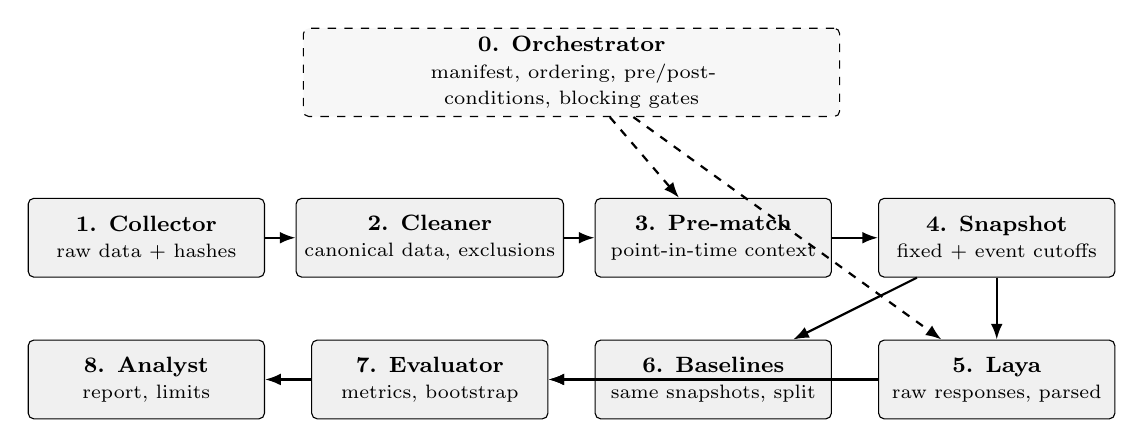
\begin{tikzpicture}[
  font=\footnotesize,
  ag/.style={draw, rounded corners=2pt, align=center, inner sep=3pt,
             minimum width=30mm, minimum height=10mm, fill=gray!12},
  ar/.style={-{Latex[length=2mm]}, thick}
]
% data plane, row 1
\node[ag] (col) at (0,0)    {\textbf{1. Collector}\\{\scriptsize raw data $+$ hashes}};
\node[ag] (cle) at (3.6,0)  {\textbf{2. Cleaner}\\{\scriptsize canonical data, exclusions}};
\node[ag] (pre) at (7.2,0)  {\textbf{3. Pre-match}\\{\scriptsize point-in-time context}};
\node[ag] (sna) at (10.8,0) {\textbf{4. Snapshot}\\{\scriptsize fixed $+$ event cutoffs}};
% row 2
\node[ag] (lay) at (10.8,-1.8) {\textbf{5. Laya}\\{\scriptsize raw responses, parsed}};
\node[ag] (bas) at (7.2,-1.8)  {\textbf{6. Baselines}\\{\scriptsize same snapshots, split}};
\node[ag] (eva) at (3.6,-1.8)  {\textbf{7. Evaluator}\\{\scriptsize metrics, bootstrap}};
\node[ag] (ana) at (0,-1.8)    {\textbf{8. Analyst}\\{\scriptsize report, limits}};
% orchestrator
\node[ag, dashed, fill=gray!6, text width=66mm] (orch) at (5.4,2.1)
  {\textbf{0. Orchestrator}\\{\scriptsize manifest, ordering, pre/post-conditions, blocking gates}};
% arrows
\draw[ar] (col) -- (cle);
\draw[ar] (cle) -- (pre);
\draw[ar] (pre) -- (sna);
\draw[ar] (sna) -- (lay);
\draw[ar] (sna) -- (bas);
\draw[ar] (lay) -- (eva);
\draw[ar] (bas) -- (eva);
\draw[ar] (eva) -- (ana);
\draw[ar, dashed] (orch) -- (pre);
\draw[ar, dashed] (orch) -- (lay);
\end{tikzpicture}
\caption{Nine-agent pipeline. Agents communicate exclusively through hashed,
versioned artifacts; the orchestrator validates pre- and post-conditions of
every step and stops the pipeline on blocking errors.}
\label{fig:pipeline}
\end{figure}

\begin{table}[t]
\centering
\small
\begin{tabular}{@{}p{3.4cm}p{5.6cm}p{5.4cm}@{}}
\toprule
\textbf{Agent} & \textbf{Role (outputs)} & \textbf{Blocking condition} \\
\midrule
Orchestrator & Manifest, ordering, run journal & Any blocking error downstream \\
Collector & Raw responses, call logs, hashes, coverage report & Bounded retries only; no transformation \\
Cleaner & Canonical data, cleaning report, exclusions & Identifier, timing, or score incoherence \\
Pre-match & Point-in-time context, source-match lists & Any feature with a future date \\
Snapshot & Fixed $+$ event snapshots, state hashes & Any failed leakage test \\
Laya & Raw responses, normalized predictions, latency, repetition audit & Invalid response isolated, never repaired \\
Baselines & Baseline distributions, fitted parameters & Any training on the final test \\
Evaluator & Per-prediction contributions, aggregates, bootstrap, calibration & No aggregation without denominator report \\
Analyst & Final report, limits, reproducible annexes & Confirmatory/exploratory separation required \\
\bottomrule
\end{tabular}
\caption{The nine agents of the reference architecture.}
\label{tab:agents}
\end{table}

Every Laya response is classified by exactly one error code:
\begin{center}
\small
\texttt{OK} \textbullet{} \texttt{NETWORK\_RETRY\_EXHAUSTED} \textbullet{}
\texttt{INVALID\_JSON} \textbullet{} \texttt{INVALID\_SCHEMA}\\
\texttt{INVALID\_PROBABILITY} \textbullet{} \texttt{INVALID\_PROBABILITY\_SUM}
\textbullet{} \texttt{MISSING\_CATEGORY}\\
\texttt{LEAKAGE\_DETECTED} \textbullet{} \texttt{CONTEXT\_TOO\_LONG}
\textbullet{} \texttt{SDK\_ERROR}
\end{center}
\noindent Network errors may be retried with bounded exponential
backoff; every attempt is logged and no retry ever replaces the original
response. Parsing, schema, and leakage failures are validity errors and are
never auto-repaired without diagnosis. Ten per-agent log files plus a shared
error log record timestamp, agent, run identifier, entity identifier, action,
status, and a short message---with no personal data; player identifiers are
pseudonymized wherever retained. The fixed execution order is collector,
cleaner, pre-match, snapshot, Laya, baselines, evaluator, analyst; each step
verifies its prerequisite artifacts and writes an output manifest with status
\texttt{validated}, \texttt{warning}, or \texttt{blocked}.

The protocol is considered \emph{executed as specified} when: a complete run
can be launched from the manifest; all artifacts are hashed and attributed;
100\,\% of snapshots pass the leakage tests; all responses are classified
valid or invalid with a code; every metric publishes its denominator; the
baselines use an equivalent temporal split; intervals are clustered by match;
the \texttt{other} and tail limitations are visible in the report; the final
test results did not modify the protocol; and a third party can reproduce at
least the primary metrics from the stored artifacts without new API calls.

\section{Experimental Status}
\label{sec:status}

This article is the stage-1 document of a registered report. The protocol
(v2.0.0), the preregistration package, and the reference implementation are
published and frozen before the final test set is collected or inspected:
preregistration at \OsfDOI{}; code at \GitHubURL{}. The pinned Laya version
and checkpoint will be recorded in the frozen experiment manifest at
execution time. Data collection, prediction, and evaluation follow after
preregistration; results will be reported in stage~2 exactly as specified
here. The reproducibility package retains: source code and commit hashes;
dependency lockfile and Python version; the complete experiment manifest;
seeds and model configurations; the exact Laya version and checkpoint hash;
SHA-256 hashes of raw and canonical data; exact questions and criteria; raw
Laya responses; snapshot-generation and metric scripts; exclusion and error
tables; the sample-size report; and the dates and time zones of all
timestamps. A reproduction must be able to restart from the raw files
without calling the external API again, except for steps explicitly marked
non-reproducible.

\section{Discussion and Limitations}
\label{sec:discussion}

The design has known limits, stated here rather than after the results.
\emph{Dependence:} snapshots of a match share one realized outcome; clustered
bootstrap mitigates but does not eliminate the resulting inferential
fragility, and event-driven snapshots are more dependent still.
\emph{Coarse categories:} the \texttt{other} bucket and the censored $21+$ and
$13+$ tails bound the interpretability of score distributions and expected
values. \emph{Live-data reality:} live statistics are published with delays
and revisions; we model availability as it actually occurred, so tier-C
snapshots may carry less information than an idealized real-time feed.
\emph{Scope:} five competitions over three seasons; nothing here supports a
universal claim about Laya, about other leagues, or about LLM-based engines
in general. \emph{Causality:} event-reaction contrasts are descriptive
associations in preregistered directions, not causal effects. \emph{Use:}
the study evaluates predictive quality only; it is not betting advice and
reports no profitability. \emph{Validity handling:} invalid responses are
counted, never repaired; a high invalidity rate can block the analysis
rather than be hidden. \emph{Sources:} public sports data can be corrected
after publication and carry license restrictions; apparent quality may
reflect coverage biases of the chosen sources. Finally, Laya's announced
characteristics are treated as unverified until confirmed in the installed
environment.

\section{Conclusion}
\label{sec:conclusion}

We presented a preregistered, multi-instant, leakage-audited protocol that
evaluates a typed AI decision engine---Laya---as a real-time probabilistic
forecaster of football outcomes, against statistical baselines receiving
identical point-in-time information, with clustered inference, multiplicity
control, and preregistered hypotheses. The design converts the standards of
probabilistic-forecast evaluation into an executable, auditable, nine-agent
pipeline whose every artifact is hashed and every aggregation publishes its
denominator. Whatever the stage-2 outcome, the protocol and its open-source
implementation provide a reusable template for evaluating probabilistic AI
systems in dynamic, information-asymmetric environments.

\section*{Acknowledgements}
This study protocol, the reference implementation, and this manuscript were
developed with the assistance of an AI system (Super Z, Z.ai) under the
direction of the author, who verified all content and takes full
responsibility for it. This disclosure follows emerging academic transparency
norms regarding the use of AI assistance in research.

\section*{Data and Code Availability}
The reference implementation (Python, SQLite) is open source under the MIT
license at \GitHubURL{}; the protocol text and this manuscript are licensed
under CC-BY 4.0. The preregistration is available at \OsfDOI{}. Raw match
data are not redistributed in the repository; their provenance, licenses, and
SHA-256 hashes are documented so that the full pipeline can be re-executed
from authorized sources. Laya is a third-party system, evaluated as-is.

\bibliographystyle{plainnat}
\bibliography{refs}

\end{document}
